\documentclass[a4paper,11pt]{report}
\usepackage[utf8]{inputenc}
\usepackage{graphicx}
\usepackage{url}
\usepackage{cite}
\usepackage{multicol}


\setlength{\topmargin}{-0.25in}
\setlength{\headheight}{0in}
\setlength{\textheight}{9.5in}
\setlength{\headsep}{0in}
\setlength{\oddsidemargin}{-0.25in}
\setlength{\evensidemargin}{-0.25in}
\setlength{\textwidth}{7.0in}


%opening
\title{{\bf Assignment-4 CS401} }
%\numberofauthors{2}
\author{Abhishek Pratap singh\\
kush@cse.iitb.ac.in}

\begin{document}
\maketitle
\tableofcontents
 \section{Scheduler level statistics}
 \subsection{Experiment 1: Load vs Context Switches}
  In this experiment on x axis no of cpu intensive process currently running on system (0..11...88)\\ .
  and reading for context switches taken for 10 seconds each time.\\
  experiment done upto maximum load handling power of system.\\
  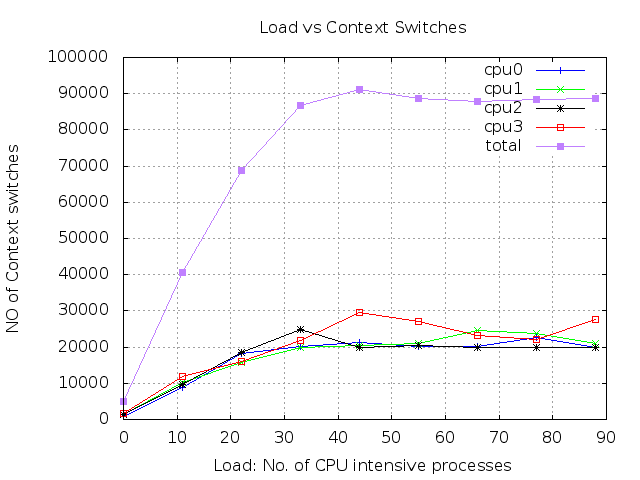
\includegraphics[scale=0.5]{loadvscs.png}
  \\{\bf conclusion:} No of context increases with load but for a particular cpu it decrease some time due load balancing among CPUs.\\
   total context switches increases with load then after some time it becomes statistically constant due to limitation of load handling capability of system and hardware.
 \subsection{Experiment 2: Run Queue length distribution per CPU}
 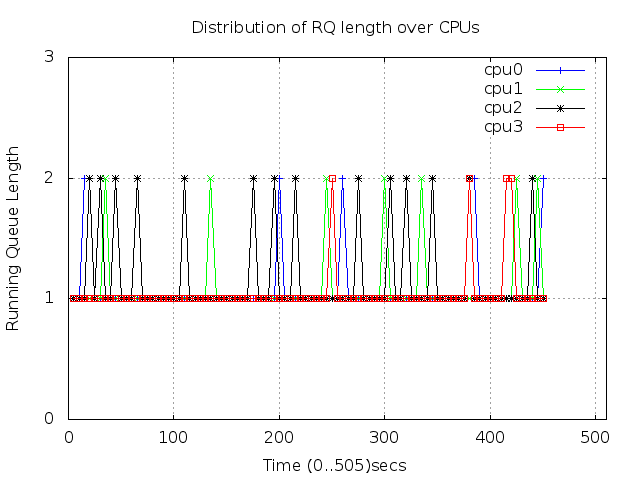
\includegraphics[scale=0.5]{rqlength.png}\\
 {\bf conclusion:} \\using this graph be can say that load is balanced , no runqueue is too long or short , all in range 1..2.
 \subsection{Experiment 3: Number of Migrations across CPUs}
 This graph with constant and low load .\\
 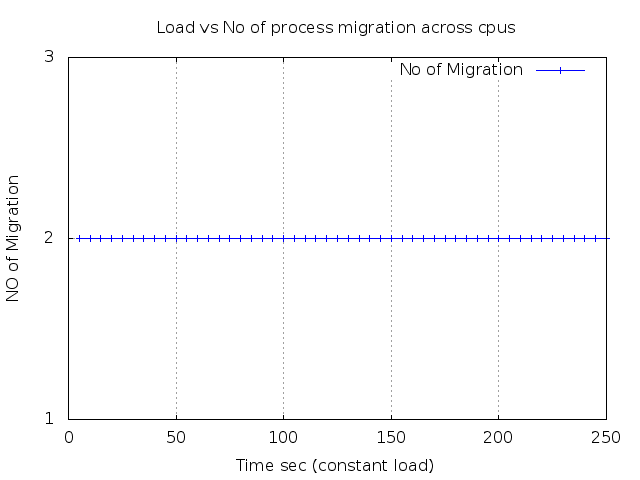
\includegraphics[scale=0.5]{mig1.png}\\
 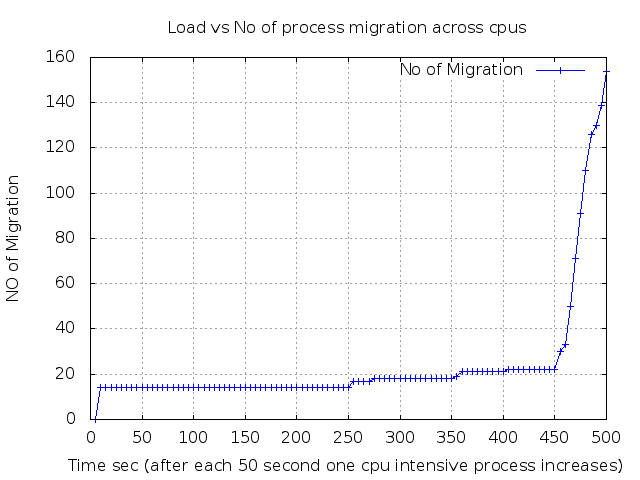
\includegraphics[scale=0.5]{mig2.png}\\
 {\bf conclusion:} \\When constant and low load on system then there is less no. of migrations because there high probability of getting same core after resuming (waking).\\
 but as load increases cpu gets busy all time , there is very low probability of getting same core because it might be busy.
 \subsection{Experiment with scheduling priorities}
 There are two cpu intensive process \\
 one with 20 nice value \\
 and other is -20 value\\
 \subsection{context switches vs time}
 There are two cpu intensive processes one with very high probability and one with very low probability .\\ 
 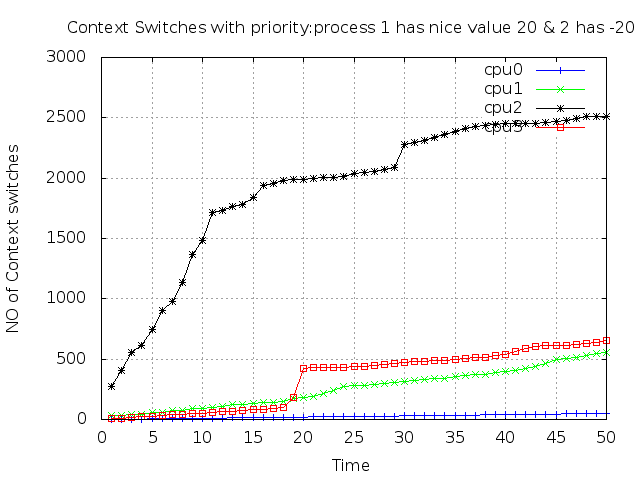
\includegraphics[scale=0.4]{priosched.png}\\
 {\bf conclusion:} \\context switches at cpu2 is far greater than other .
 \subsection{No. of migration}
  \subsubsection{Process with high probability}
  It didnt migrate to other cpus .\\
 \subsubsection{Process with low probability}
 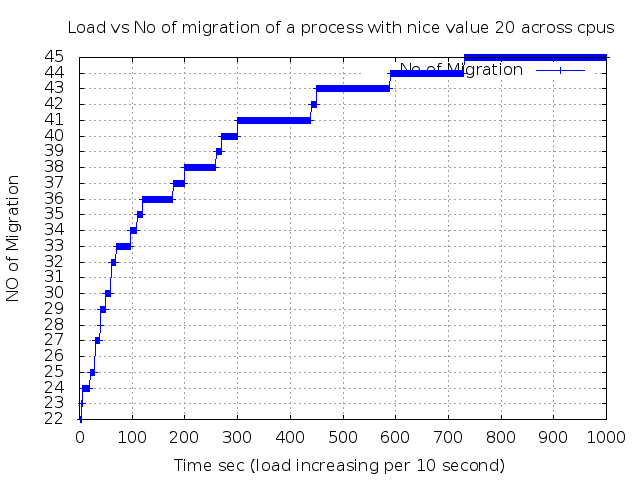
\includegraphics[scale=0.5]{miglow.png}\\
  {\bf conclusion:} \\Process with low priority has very oftenly preempt , and sheduler gives less preference to it so when any core is available scheduler schedules it so it migrate to other cpus oftenlly.
 \section{Process level Statistics}
 \subsection{Number of context switches}
 \subsubsection{Meory intensive Process}
 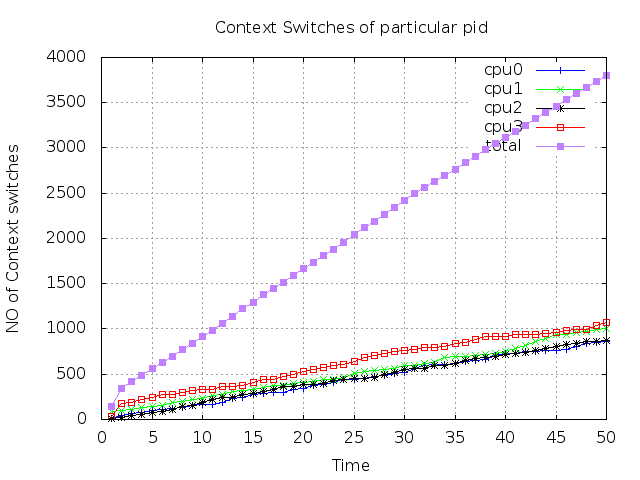
\includegraphics[scale=0.5]{pidcs.png}\\
 \subsubsection{CPU intensive Process}
 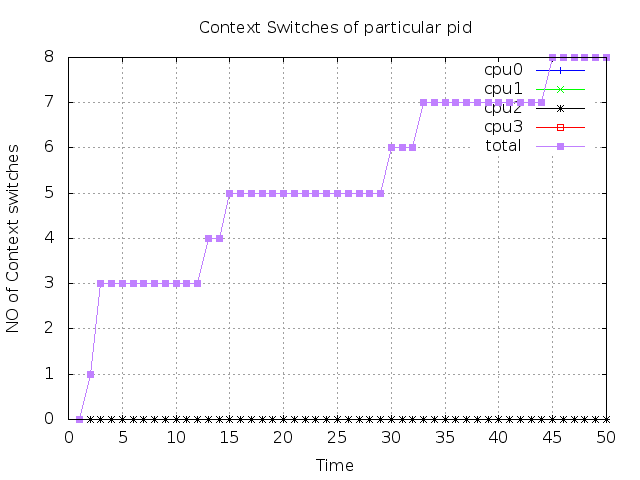
\includegraphics[scale=0.5]{pidcpucs.png}\\
 {\bf conclusion:}\\ Memory intensive process changes state regularly to procees i/o so it sees lot of context switches.\\
 but in case of CPU intensive process scheduler changes state not process itself thats why it sees few context switches in same condition. 
 
 \subsection{Variation in dynamic priority of the process}
 I tried it with differnt combination but all type priorities were constant througout all experiment . i think something is missing.
 \subsection{CPU mapping distribution of process}
  \subsubsection{CPU intensive process}
  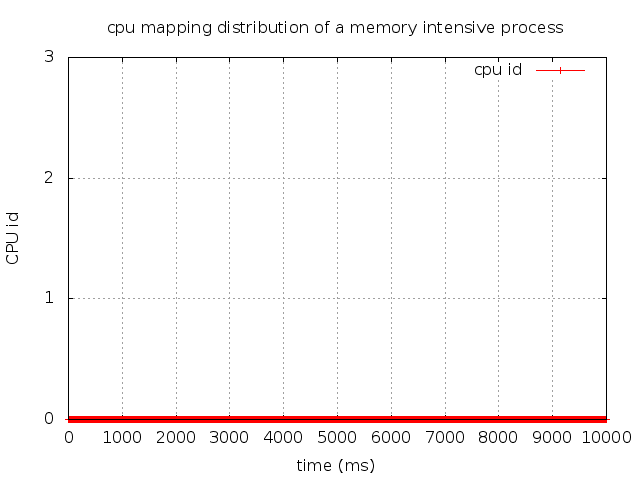
\includegraphics[scale=0.5]{memcurr_cpu.png}\\
  {\bf conclusion:} At low load cpu intensive process keep executing to a particular core until scheduler switches its state
  so it sees very less migration.\\
  {\bf In this case no migration occured}
  \subsubsection{Memory intensive Process}
  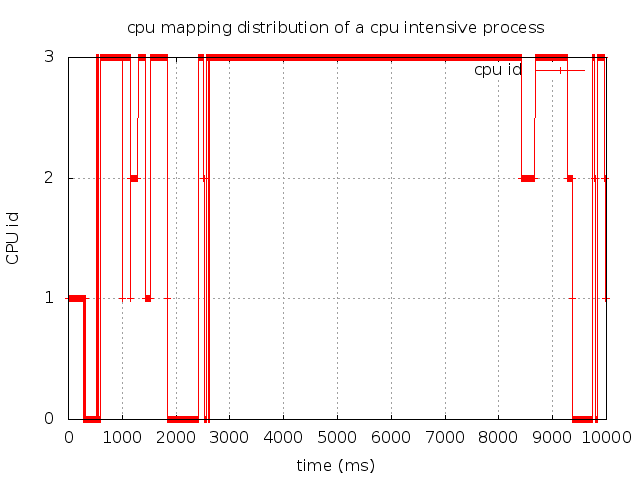
\includegraphics[scale=0.5]{curr_cpu.png}\\ 
  {\bf conclusion:} \\At normal load there are lot of migration because it is a memory intensive process so it goes into i/o-wait state and then at resuming time some times it doesnt get same cpu.\\
  due to changing state a lot , it sees migrations . 
 \subsection{Experiments with CPU affinity of process}
 \subsubsection{CPU intensive process with core affinity}
 In this case process remains on same cpu and very less context switches.\\
 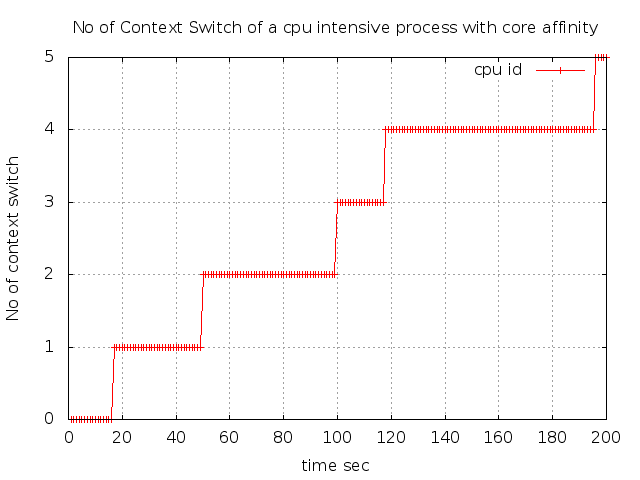
\includegraphics[scale=0.5]{csaff.png}\\
 {\bf conclusion:} \\Process follows affinity and doesnt migrate to other cpus even load increase , as we have seen behaviour of a cpu intensive process at normal constant load in 0.2.3 section , according to that section graph cpu intensive migrate to other cpus rarely.
 \subsubsection{Memory intensive process with core affinity}
 Memory intensive process goes to other cores sometimes even it pinned to core 2.\\
 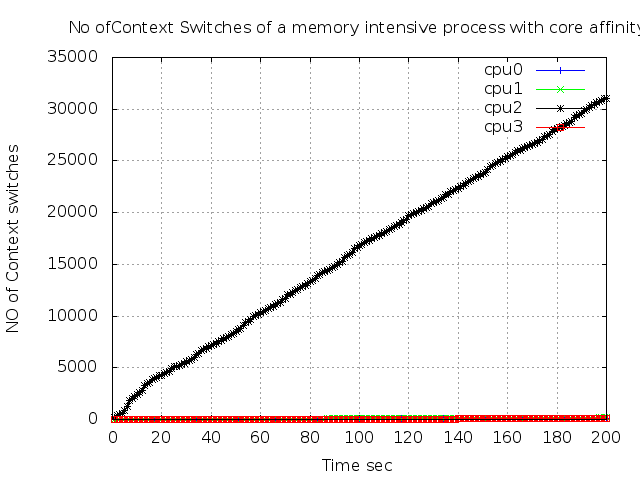
\includegraphics[scale=0.5]{memlast.png}\\
 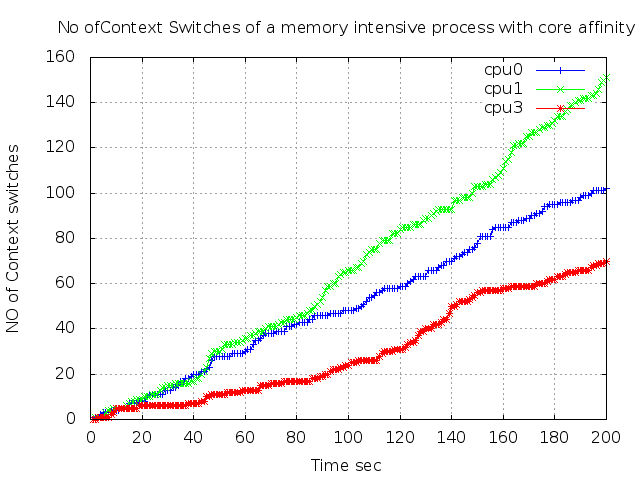
\includegraphics[scale=0.5]{memlast2.png}\\
 This second graph is a part of first graph in this section, it shows context switches to other cpu (other than pinned one). 
\\{\bf conclusion:} \\This is memory intensive process so it changes state regularlly , in some cases at the time of resuming cpu on which it is pinned is not free (may be occupied by high probability process) so scheduler switches it to other cpus too.   
\end{document}
